% This is a variation of the NeurIPS'24 format
\documentclass{article}
\usepackage[final]{adrl}

\usepackage[utf8]{inputenc} % allow utf-8 input
\usepackage[T1]{fontenc}    % use 8-bit T1 fonts
\usepackage{hyperref}       % hyperlinks
\usepackage{url}            % simple URL typesetting
\usepackage{booktabs}       % professional-quality tables
\usepackage{amsfonts}       % blackboard math symbols
\usepackage{amsmath}        % align, cases, ...
\usepackage{nicefrac}       % compact symbols for 1/2, etc.
\usepackage{microtype}      % microtypography
\usepackage{xcolor}
\usepackage{graphicx}
\usepackage{float}          % [H] float placement
\usepackage{algorithm}
\usepackage{algpseudocode}

\graphicspath{{figures/}{../figures/}{../agents/comparison/}}

\title{How Far Back Must the Gradient Reach?\\
Truncated BPTT Length and Memory in PPO on MiniGrid}
\author{Anh Khoa Pham \\ \url{github.com/khoaphamanh/rl_project}}

\begin{document}

\maketitle
\begin{abstract}
    A recurrent policy can only use a memory that its gradient has taught it to
    write. We measure how far back that gradient has to reach on
    \texttt{MiniGrid-MemoryS17Random-v0}, a partially observable task in which a
    cue visible only at one end of a corridor decides which prong of a
    T-junction at the far end is correct. One PPO pipeline is run with a
    memoryless MLP and with a GRU whose truncated backpropagation-through-time
    (TBPTT) window $L$ is varied over $\{1, 4, 8, \infty\}$, and each arm is
    tuned by its own 50-trial Optuna study over identical ranges at an identical
    fixed budget. The outcome is a sharp threshold between $L=4$ and $L=8$:
    $L \in \{8, \infty\}$ reach $1.000 \pm 0.000$ success, while $L \in \{1,4\}$
    and the MLP stay at chance. Carrying the hidden state forward is therefore
    not the deciding factor, since every GRU arm does that; the gradient itself
    has to span the interval between cue and decision. Truncating is also not
    cheaper in time: full BPTT was the best-scoring arm and the fastest GRU arm
    ($1.3$\,h vs.\ $2.6$\,h at $L=1$), and paid only in VRAM.
\end{abstract}

\section{Introduction}

In a partially observable task the optimal action depends on information that
has left the observation \citep{pomdp}. The usual remedy is a recurrent policy
carrying a hidden state $h_t$ forward \citep{drqn, recurrentbaseline}, and the
usual practical concession is to truncate the backward pass to $L$ steps
\citep{tbptt, r2d2}, because full backpropagation through time \citep{bptt}
costs activation memory linear in sequence length. That concession is usually
made silently, with $L$ inherited from whatever codebase a project starts from.
We ask what it buys and what it costs:

\begin{enumerate}
    \item \textbf{How far back must the gradient reach} before a policy solves a
    task that a memoryless policy provably cannot? Carrying $h_t$ forward is free
    regardless of $L$, so is a short window enough to \emph{learn} what to store,
    or must the gradient span cue and decision?
    \item \textbf{What does that reach cost} in wall-clock time and memory? A
    shorter window is intuitively cheaper; we check whether it is.
\end{enumerate}

The setting is \texttt{MiniGrid-MemoryS17Random-v0} \citep{minigrid}
(Figure~\ref{fig:setup}, top). The agent sees a $7 \times 7$ egocentric patch,
so at the junction the observation is identical whichever answer is correct: a
memoryless policy is capped at chance, and the gap between $0.5$ and $1.0$
success is exactly the memory a run has acquired. We hold one PPO
\citep{ppo} pipeline fixed and change only the encoder (MLP or GRU
\citep{gru}) and, for the GRU, $L \in \{1,4,8,\infty\}$. Since hyperparameters
and outcomes are tightly coupled in RL \citep{hyperparamsrl, whatmatters}, every
arm gets an independent Optuna \citep{optuna} study over identical ranges and an
identical non-searchable budget.

\section{Related Work}

\citet{drqn} showed that a recurrent value function recovers performance under
flickering observations, and \citet{recurrentbaseline} found that a carefully
implemented recurrent model-free agent is a strong baseline across many POMDPs,
with details such as how sequences are cut and how hidden states are seeded
mattering more than the algorithm. Attention-based memories \citep{gtrxl} and dedicated
benchmarks \citep{popgym} pursue the same question with larger machinery.
Truncated BPTT \citep{tbptt} bounds the cost of training such policies, and R2D2
\citep{r2d2} studies the artefacts it introduces, proposing the stored-state and
burn-in recipe now in common use; our chunking follows the same stored-state
principle, but where R2D2 fixes $L$ and corrects for it, we vary $L$ and ask
where the task stops being solvable. Finally,
\citet{implementationmatters, whatmatters} document how much of the reported
difference between deep RL methods comes from tuning rather than from the
method, and \citet{hyperparamsrl} recommend the kind of per-method tuning
protocol at a stated budget that we follow below.

\begin{figure}[t]
    \centering
    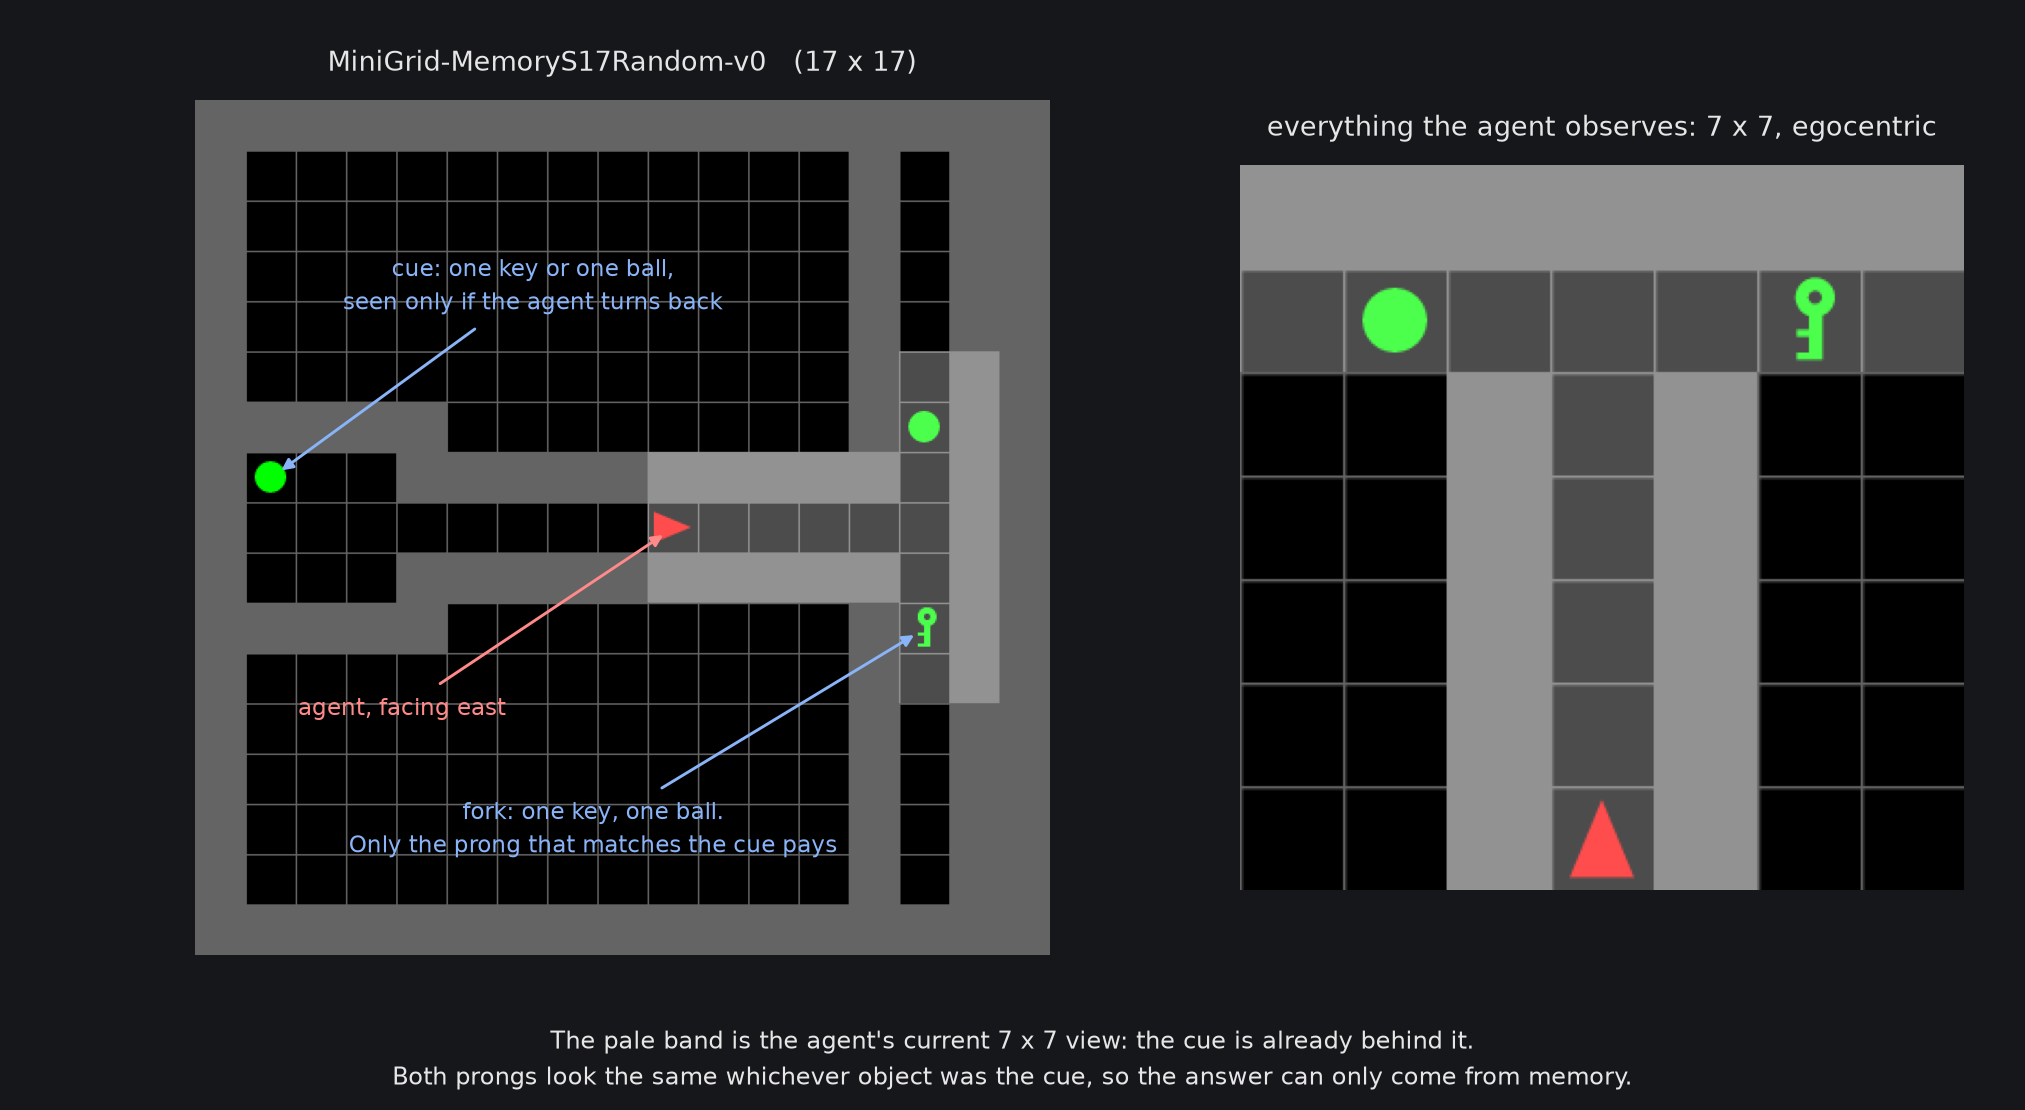
\includegraphics[width=1.0\linewidth]{task_memory_s17.png}\\[6pt]
    
\includegraphics[width=1.0\linewidth]{model_architecture.png}
    \caption{\textbf{Top:} \texttt{MiniGrid-MemoryS17Random-v0}. A cue (key or
    ball) sits in the west room; the corridor forks into a T with a key at one
    prong and a ball at the other, and success requires reaching the prong
    matching the cue. The agent spawns at a random corridor position facing away
    from the cue, so the information must be actively sought.
    \textbf{Bottom:} one shared encoder feeding a linear actor head over the $7$
    actions and a linear critic head. The encoder is the only part that differs
    between arms.}
    \label{fig:setup}
\end{figure}

\section{Approach}

\paragraph{Task and network.} The environment is a POMDP: a
$7 \times 7 \times 3$ egocentric view (object, colour and state index per cell),
one-hot encoded per channel into $980$ features, and $7$ discrete actions.
Reward is MiniGrid's $1 - 0.9 \cdot \text{step\_count}/\text{max\_steps}$ on
success and $0$ otherwise, with \texttt{max\_steps} set to the rollout length
$T=361$. Both arms share the actor-critic skeleton of Figure~\ref{fig:setup}
(bottom) and differ only in the encoder $f_\theta$, which maps $(B,T,7,7,3)$ to
$(B,T,H)$: the MLP applies $n \in \{1,\dots,4\}$
\texttt{Linear}+\texttt{ReLU} blocks to each timestep independently, so no state
crosses the sequence and its gradient spans one step, while the GRU \citep{gru}
is a single layer of width $H$ carrying $h_t$ forward, so an observation from a
hundred steps ago can still be present at the decision.

\paragraph{PPO.} One iteration collects $W=32$ workers $\times\ T=361$ steps,
computes advantages by GAE \citep{gae},
\begin{equation}
    \delta_t = r_t + \gamma V(s_{t+1})(1 - d_t) - V(s_t), \qquad
    \hat{A}_t = \delta_t + \gamma \lambda (1 - d_t) \hat{A}_{t+1}, \qquad
    \hat{R}_t = \hat{A}_t + V(s_t),
    \label{eq:gae}
\end{equation}
standardises $\hat{A}$ once over the whole rollout (returns $\hat{R}$ keep their
own scale, being what the critic must predict), and takes up to
$n_{\text{epochs}}=3$ shuffled passes minimising
\begin{equation}
    \label{eq:loss}
    \mathcal{L} = -\,\mathbb{E}_t\!\left[\min\!\left(\rho_t \hat{A}_t,\;
    \mathrm{clip}(\rho_t, 1-\epsilon, 1+\epsilon) \hat{A}_t\right)\right]
    + c_v \mathbb{E}_t\!\left[(V_\theta(s_t) - \hat{R}_t)^2\right]
    - c_e \mathbb{E}_t\!\left[\mathcal{H}(\pi_\theta(\cdot \mid s_t))\right],
\end{equation}
with $\rho_t = \exp(\log \pi_\theta(a_t|s_t) - \log \pi_{\theta_{\text{old}}}(a_t|s_t))$
\citep{ppo}. Every expectation covers real timesteps only, since chunks are
padded inside a minibatch and padding never enters the loss, and gradients are
clipped to \texttt{max\_grad\_norm} before each Adam \citep{adam} step.

\paragraph{The knob under study.} Before the update the rollout is cut at every
episode boundary \emph{and} every $L$ steps (Algorithm~\ref{alg:chunk}). A chunk
beginning mid-episode is seeded with the hidden state the rollout already
recorded there, so the forward pass still sees the whole episode and
\textbf{only the backward pass is shortened}. This isolates the quantity of
interest: all GRU arms carry identical information forward and differ only in how
far credit assignment reaches. Setting $L=\infty$ (full BPTT) cuts at episode
boundaries only. Note that a smaller $L$ yields \emph{more, shorter} sequences,
which is why truncating does not automatically save time.

\begin{algorithm}[H]
    \caption{One PPO iteration with truncation length $L$. {\color{orange}The
    highlighted line is the only difference between arms.}}
    \label{alg:chunk}
    \begin{algorithmic}[1]
        \Require policy $\pi_\theta$, critic $V_\theta$, workers $W$, steps $T$, truncation length $L$
        \State $\mathcal{B} \gets$ rollout of $W \times T$ transitions, recording $(o_t, a_t, \log \pi_t, V_t, r_t, d_t, h_t)$
        \State compute $\hat{A}, \hat{R}$ by GAE (Eq.~\ref{eq:gae}); standardise $\hat{A}$ over $\mathcal{B}$
        \State {\color{orange}$\mathcal{S} \gets \textsc{Chunk}(\mathcal{B})$: split at episode boundaries \textbf{and} every $L$ steps, seeding each chunk with its recorded $h$}
        \For{epoch $=1 \dots n_{\text{epochs}}$, minibatch $\mathcal{M} \subset \mathcal{S}$ (shuffled, padded)}
            \State forward $f_\theta$ over $\mathcal{M}$ from the stored $h_0$, evaluate Eq.~\ref{eq:loss} on non-padding steps
            \State backpropagate ($\le L$ steps through the recurrence), clip gradient norm, Adam step
        \EndFor
    \end{algorithmic}
\end{algorithm}

\paragraph{Tuning protocol.}
\label{sec:hpo}
Each arm gets one Optuna study \citep{optuna} of $50$ trials with a TPE sampler
\citep{tpe} seeded at $42$. A trial trains the \emph{same five seeds}
$[0,15,12,97,98]$ for $1000$ iterations ($\approx 11.6$M environment steps per
seed) and evaluates each on $50$ fixed mazes from a held-out evaluation seed.
Trials are ranked by $\mathrm{mean}_s[\text{return}_s] -
\mathrm{std}_s[\text{return}_s]$, the spread taken across seeds and never across
the episodes of one run, since the per-episode return is bimodal and within-run
spread would merely restate the success rate. Nine parameters are searched over
ranges identical for both encoders, plus the MLP's depth
(Appendix~\ref{app:params}). Nothing that buys compute is searchable: epochs,
iterations, workers, rollout length and $L$ are fixed, and each $L$ is its own
study, so no sampler ever ranks one truncation length against another. The
minibatch size is instead resolved per run by probing candidates from $4096$
downwards and keeping the largest that fits in VRAM, so every run is measured at
the same memory budget and the winning size is itself a result.

\section{Experiments}

\paragraph{Setup.} Five studies were run (MLP; GRU at $L \in \{1,4,8\}$ and full
BPTT), that is $250$ training runs and roughly $236$ GPU-hours, on one NVIDIA
RTX 3060 Laptop GPU (12\,GB VRAM) with an AMD Ryzen 9 7950X, using PyTorch
\citep{pytorch}, Gymnasium \citep{gymnasium} and MiniGrid \citep{minigrid}.
Every number below is the winning trial of that study, averaged over its five
seeds, with $\pm$ denoting the standard deviation across seeds.

\begin{table}[t]
    \centering
    \caption{Winning trial per study. \emph{steps} is the mean evaluation
    episode length, \emph{minibatch} the size the VRAM probe settled on, and
    \emph{time} the wall-clock training time of that trial for all five seeds.}
    \label{tab:results}
    \small
    \begin{tabular}{llccccc}
        \toprule
        arm & encoder & return & success rate & steps & minibatch & time \\
        \midrule
        \texttt{MLP} & MLP (memoryless) & $0.556 \pm 0.029$ & $0.592 \pm 0.027$ & $24.3$ & $1024$ & $1.3$\,h \\
        \texttt{GRU} $L{=}1$ & GRU & $0.573 \pm 0.064$ & $0.588 \pm 0.068$ & $9.8$ & $4096$ & $2.6$\,h \\
        \texttt{GRU} $L{=}4$ & GRU & $0.492 \pm 0.001$ & $0.500 \pm 0.000$ & $7.0$ & $4096$ & $1.6$\,h \\
        \texttt{GRU} $L{=}8$ & GRU & $\mathbf{0.958 \pm 0.004}$ & $\mathbf{1.000 \pm 0.000}$ & $16.8$ & $4096$ & $2.0$\,h \\
        \texttt{GRU} full BPTT & GRU & $\mathbf{0.958 \pm 0.002}$ & $\mathbf{1.000 \pm 0.000}$ & $16.8$ & $512$ & $\mathbf{1.3}$\,\textbf{h} \\
        \bottomrule
    \end{tabular}
\end{table}

\begin{figure}[t]
    \centering
    
\includegraphics[width=\linewidth]{compare_curves.pdf}
    \caption{Training curves of the winning trial of each study: means over the
    five seeds, bands at $\pm 1$ standard deviation across seeds, dashed line at
    chance ($0.5$). The two solving arms separate well before iteration $400$;
    the three failing arms sit on the chance line for the whole budget.}
    \label{fig:curves}
\end{figure}

\paragraph{The cut-off is sharp and sits between $L=4$ and $L=8$.}
Table~\ref{tab:results} and Figure~\ref{fig:curves} answer the first question
categorically rather than gradually. The arms with $L \in \{8, \infty\}$ solve
the task, at $1.000$ success on all five seeds and return $0.958$, while $L=4$
($0.500$), $L=1$ ($0.588$) and the MLP ($0.592$) never beat a coin flip, and no
setting produced an intermediate score such as $0.75$. Carrying $h$ forward is
therefore not what matters, because every GRU arm does that identically,
including the ones that fail; what separates them is whether
the gradient reaches back to the observation that filled $h$, and four steps is
not far enough while eight is. Reaching further than $8$ adds nothing, since
full BPTT matches $L=8$ within noise.

\paragraph{Why eight steps suffice for a seventeen-step solution.} The
$16.8$-step episode is the wrong comparison. Truncation never limits how long the
policy can \emph{remember}, since the forward pass is untouched and every arm
carries $h$ across the whole episode; it limits only whether the encoder can
\emph{learn to write} the cue into $h$, which requires the cue observation and
the rewarded decision to fall inside the same chunk. The interval that must fit
inside $L$ is therefore the \emph{gap}, the number of actions between the agent's
last sighting of the cue and its choice at the fork, and not the episode: every
step before the sighting needs no memory. We measured this gap by breadth-first
search over the environment's own state and visibility model. It is governed by
the corridor length, redrawn at every reset
($\texttt{hallway\_end} \in \{4,\dots,14\}$), together with the fact that the
$7 \times 7$ view reaches six tiles back from the junction: the shortest
attainable gap is $2$ for corridors up to $6$ and then grows linearly to $12$ at
$14$. A gap of at most $8$ is attainable in $62\%$ of mazes, one of at most $4$
in only $26\%$, and no maze at all can be solved from the spawn within four
actions, the minimum being five. Replaying the trained checkpoints over the $50$
evaluation mazes confirms the consequence: cue and decision share a chunk in
$16\%$ of the $L=8$ agent's episodes and in $0$ of $50$ of the $L=4$ agent's.
Two further facts explain why partial coverage is sufficient. Because a GRU
applies the same weights at every timestep, the write rule acquired in short-gap
episodes transfers to every distance at no cost, so $L=8$ need only cover part of
the maze distribution rather than its mean; and GAE, computed over the full
rollout before the split (Eq.~\ref{eq:gae}), carries reward credit across chunk
boundaries irrespective of $L$, so truncation removes the gradient through $h$
and not the reward signal. The $L=4$ arm, meanwhile, has an easier target
available: a blind dash reaches the fork within four actions in $26\%$ of mazes,
pays $0.5$, and removes the look-back behaviour on which its only learning route
depends.

\paragraph{The failing arms have solved a different problem.} Mean episode
length separates two policies more cleanly than return does. At $\approx 16.8$
steps the solving arms take the detour (turn back, look, return to the fork) and
pay the small step cost that keeps their return at $0.958$ rather than $1.0$. At
$7.0$ steps the $L=4$ arm walks straight to the fork and always picks the same
side, the upper prong on four seeds and the lower on the fifth, on
\emph{every} maze. The upper prong is correct in exactly $25$ of the $50$
evaluation mazes, so any fixed side scores exactly $25/50$; its across-seed
spread of $0.000$ is arithmetic, not convergence. Sub-threshold arms are thus not partially remembering but have settled in a
stable memory-free optimum, which is easy to reach because the detour costs
reward immediately and pays nothing until the memory works. The $L=1$ arm
($9.8$ steps) does the same less tidily and the MLP ($24.3$ steps) wanders
before guessing; the small excess of these two above $0.5$ is sampling noise
over $50$ mazes, since their across-seed spreads ($\pm 0.07$ and $\pm 0.03$)
cover chance comfortably. All three are flat from about iteration $50$ onwards
in Figure~\ref{fig:curves}, so a larger budget would not rescue them.

\paragraph{The reach costs memory, not time.} Full BPTT is the fastest GRU arm
at $1.3$\,h, matching the memoryless MLP, against $1.6$\,h ($L=4$), $2.0$\,h
($L=8$) and $2.6$\,h ($L=1$). The intuition that truncation saves time is wrong
at fixed rollout size: sequences per epoch scale as $\lceil T/L \rceil$, so
halving $L$ roughly doubles the number of padded, kernel-launch-bound minibatch
sequences, and the per-sequence saving in the backward pass does not compensate
(the extremes are the clean comparison, as the middle two arms also differ in
width). Full BPTT is earlier as well, reaching $0.95$ success at a median of
$370$ iterations against $640$ for $L=8$. What it pays is VRAM: the probe settles
at a minibatch of $512$ against $4096$ for $L=8$, an $8\times$ difference on the
same 12\,GB GPU. The recommendation on this task is therefore full BPTT, with
$L=8$ as the fallback on a smaller GPU; below $L=8$ one does not get a cheaper
solution but the MLP's guessing policy at GRU prices.

\section{Discussion}

On MemoryS17Random the gradient must reach back between $4$ and $8$ steps, with
no partial credit on either side of that boundary and no benefit beyond it, and
the reach costs activation memory ($8\times$ smaller minibatches) but not
wall-clock time, since hard truncation was the slowest configuration we ran. The
control that makes this interpretable is the stored-state chunking: every GRU
arm carries the identical hidden state forward, so the collapse at $L \le 4$ is
attributable to credit assignment and not to information availability. The
per-arm tuning protocol was essential rather than cosmetic, since with $50$
trials each and a variance-penalised objective the failure of $L \in \{1,4\}$
cannot be dismissed as an unlucky learning rate. Our cost intuition did not
survive: we expected a score/compute trade-off along $L$ and found the
best-scoring setting to be the cheapest in time as well, so truncation is best
understood here as a memory concession rather than a speed optimisation.

\paragraph{Limitations and future work.} This is one task, one recurrent
architecture and one algorithm. The threshold is a property of
MemoryS17Random, and we did not resolve $L \in \{5,6,7\}$, so it is bracketed
rather than located. Five seeds separate $0.5$ from $1.0$ safely but do not support
fine claims such as the $0.556$ versus $0.573$ ordering of two chance-level
arms, and evaluation uses $50$ fixed mazes from a single seed. Three extensions
follow directly: sweep $L \in \{5,6,7\}$ and control the corridor length
directly instead of leaving it to the environment's randomisation, which would
locate the threshold rather than bracket it and test the gap account of
Section~4 causally; add R2D2-style burn-in \citep{r2d2}, which
would tell us whether a short window can be made to behave like a long one, in which case the threshold is about optimisation rather
than the gradient path itself; and repeat the protocol with an LSTM
\citep{lstm} and a small transformer \citep{gtrxl}, where the analogous knob is
the attention window.

% Everything from this point on does not count towards your page count
\newpage
\bibliography{references}
\bibliographystyle{plainnat}

\newpage
\appendix
\section{Search space and winning hyperparameters}
\label{app:params}

Table~\ref{tab:params} gives the search space, identical for both encoders, and
the configuration of the winning trial of each study, that is the settings
behind every number in Table~\ref{tab:results}. The tuned values are similar
across the solving and the failing GRU arms (learning rates within a factor of
$1.4$, comparable discounting), so the outcome is not explained by one study
finding a special corner of the space. The one visible pattern is the MLP's much
larger entropy coefficient and value weight, consistent with a run that never
finds a deterministic solution to commit to.

\begin{table}[h]
    \centering
    \caption{Search space (identical ranges per encoder) and the winning
    configuration per study. \texttt{score} is $\mathrm{mean}_s -
    \mathrm{std}_s$ of the evaluation return over the five seeds, the quantity
    Optuna maximised. Fixed, never-searched settings: $n_{\text{epochs}}=3$,
    $1000$ iterations, $32 \times 361$ rollout, and $L$ itself.}
    \label{tab:params}
    \small
    \begin{tabular}{llccccc}
        \toprule
        parameter & range & MLP & $L{=}1$ & $L{=}4$ & $L{=}8$ & full BPTT \\
        \midrule
        winning trial & & 3 & 47 & 40 & 25 & 36 \\
        \texttt{lr} & $10^{-5}$--$10^{-2}$, log & $6.65\!\cdot\!10^{-4}$ & $1.53\!\cdot\!10^{-3}$ & $1.48\!\cdot\!10^{-3}$ & $1.35\!\cdot\!10^{-3}$ & $1.82\!\cdot\!10^{-3}$ \\
        \texttt{gamma} & $0.99$--$0.9999$ & $0.9917$ & $0.9968$ & $0.9962$ & $0.9940$ & $0.9968$ \\
        \texttt{gae\_lambda} & $0.9$--$0.99$ & $0.90$ & $0.95$ & $0.90$ & $0.98$ & $0.96$ \\
        \texttt{clip\_eps} & $0.1$--$0.3$ & $0.26$ & $0.19$ & $0.10$ & $0.13$ & $0.25$ \\
        \texttt{entropy\_coef} & $10^{-4}$--$10^{-1}$, log & $7.03\!\cdot\!10^{-2}$ & $9.27\!\cdot\!10^{-4}$ & $3.30\!\cdot\!10^{-4}$ & $5.11\!\cdot\!10^{-3}$ & $9.56\!\cdot\!10^{-3}$ \\
        \texttt{value\_coef} & $0.01$--$1.0$, log & $0.854$ & $0.120$ & $0.028$ & $0.128$ & $0.089$ \\
        \texttt{wd} & $10^{-8}$--$10^{-2}$, log & $6.72\!\cdot\!10^{-7}$ & $1.60\!\cdot\!10^{-7}$ & $2.74\!\cdot\!10^{-7}$ & $1.21\!\cdot\!10^{-8}$ & $2.87\!\cdot\!10^{-8}$ \\
        \texttt{max\_grad\_norm} & $0.1$--$2.0$, log & $0.134$ & $1.152$ & $1.226$ & $0.304$ & $0.500$ \\
        \texttt{hidden\_size} & $32$--$512$, step $8$ & $360$ & $216$ & $360$ & $480$ & $280$ \\
        \texttt{n\_layers\_mlp} & $1$--$4$ (MLP only) & $2$ & & & & \\
        \midrule
        \texttt{score} & & $0.527$ & $0.509$ & $0.491$ & $0.955$ & $\mathbf{0.956}$ \\
        \bottomrule
    \end{tabular}
\end{table}

\newpage
\section*{Checklist}
This checklist is not mandatory, but can help you set up your project in a reproducible manner.
Options for filling it out are:
\answerYes{}
\answerNo{}
\answerNA{}
\begin{enumerate}

\item General points:
\begin{enumerate}
  \item Do the main claims made in the abstract and introduction accurately reflect your contributions and scope?
    \answerYes{} The claims are limited to one task, one recurrent architecture and the four truncation lengths actually run.
  \item Did you cite all relevant related work?
    \answerYes{} See Section~2 (recurrent policies in POMDPs, truncated BPTT and stored states, tuning protocols in RL).
  \item Did you describe the limitations of your work?
    \answerYes{} Section~5: single task and architecture, threshold bracketed rather than located, five seeds, one evaluation seed.
  \item Did you include a discussion of future work?
    \answerYes{} Section~5, three concrete extensions.
\end{enumerate}

\item If you are including theoretical results...
\begin{enumerate}
  \item Did you state the full set of assumptions of all theoretical results?
    \answerNA{} The report is purely empirical.
	\item Did you include complete proofs of all theoretical results?
    \answerNA{}
\end{enumerate}

\item If you ran experiments (e.g. for benchmarks)...
\begin{enumerate}
  \item Did you include the code, data, and instructions needed to reproduce the main experimental results (either in the supplemental material or as a URL)?
    \answerYes{} Code, the exact command per study, and the finished Optuna studies with the winning checkpoints are at \url{https://github.com/khoaphamanh/rl_project}.
  \item Did you specify all the training details (e.g., data splits, hyperparameters, how they were chosen)?
    \answerYes{} Protocol in Section~3; search space and selected values in Appendix~\ref{app:params}.
  \item Did you run at least 10 repetitions of your method?
    \answerNo{} Each configuration was trained on five seeds $[0,15,12,97,98]$, the same five in every trial of every study, for $250$ training runs and $\approx 236$ GPU-hours. The measured effect ($0.500$ vs.\ $1.000$ success, across-seed std $\le 0.004$ on the solving arms) is far larger than the seed noise, so more repetitions would not change the conclusion; a finer comparison between the two chance-level arms would need them.
  \item Did you report error bars (e.g., with respect to the random seed after running experiments multiple times)?
    \answerYes{} All tables report mean $\pm$ std across seeds, Figure~\ref{fig:curves} shades $\pm 1$ std, and the tuning objective is itself mean minus one std across seeds.
  \item Did you include the total amount of compute and the type of resources used (e.g., type of GPUs, internal cluster, or cloud provider)?
    \answerYes{} Section~4: one RTX 3060 Laptop GPU (12\,GB), Ryzen 9 7950X, $\approx 236$ GPU-hours in total.
\end{enumerate}

\item If you are using existing assets (e.g., code, data, models) or curating/releasing new assets...
\begin{enumerate}
  \item If your work uses existing assets, did you cite the creators?
    \answerYes{} MiniGrid \citep{minigrid}, Gymnasium \citep{gymnasium}, Optuna \citep{optuna} and PyTorch \citep{pytorch} are cited where used.
  \item Did you make sure the license of the assets permits usage?
    \answerYes{} All four are permissively licensed (MIT/BSD-style) and used unmodified.
  \item Did you reference the assets directly within your code and repository?
    \answerYes{} They are pinned in \texttt{requirements.txt} and named in the repository README.
\end{enumerate}
\end{enumerate}
\end{document}
